%! Author = danielmendes
%! Date = 29.11.24

\chapter{Indexierung und Einfluss auf die Performance}

\section{Grundlagen der Indexierung}\label{sec:grundlagen-der-indexierung}

Das folgende Thema befasst sich mit der Indexierung und den damit verbundenen Performance-Optimierungen, die näher erläutert werden.
Zunächst betrachten wir die Grundlagen der Indexierung, anschließend die verschiedenen Arten von Indizes und schließlich deren Auswirkungen auf die Performance.

Indizes (oder auch Indexes) sind Datenstrukturen, die von Speicher-Engines (engl. storage engines) verwendet werden, um unter anderem Zeilen schneller zu finden.
Sie haben einen großen Einfluss auf die Performance der Datenbank und werden umso wichtiger, je größer die Datenbank wird.
Weniger ausgelastete Datenbanken können ohne ordnungsgemäße Indizes gut funktionieren, aber die Leistung kann rapide sinken, wenn die Datenmenge wächst.
Wenn ein solches Problem auftritt, ist die Index-Optimierung oft der effektivste Weg, die Abfrageleistung zu verbessern.
Um wirklich optimale Indizes zu erstellen, ist es häufig notwendig, Abfragen umzuschreiben.
Wie genau Indizes erstellt werden müssen, wird im weiteren Verlauf der Arbeit betrachtet.

Um die Funktionsweise eines Indexes zu verdeutlichen, betrachten wir ein Beispiel aus einem wissenschaftlichen Fachbuch.
Am Ende solcher Bücher gibt es meist ein Stichwortverzeichnis oder Register.
Dieses Register besteht aus einer alphabetisch geordneten Liste von Begriffen, Themen und Stichworten.
Möchte man einen Begriff nachschlagen, sucht man ihn in der Liste und erhält die Seitenzahlen, auf denen er vorkommt.
In MySQL verwendet die Storage-Engine Indizes auf ähnliche Weise.
Sie durchsucht die Datenstruktur des Indexes nach einem Wert.
Wird ein Treffer gefunden, kann die Engine die Zeile ermitteln, die den Treffer enthält.
Betrachten wir dazu folgendes Beispiel:
\begin{lstlisting}[language=SQL,caption=Variationen,label=select-query-customer]
SELECT name FROM customer WHERE cust_id = 7;
\end{lstlisting}

Es gibt einen Index auf der Spalte \texttt{cust\_id}, sodass MySQL diesen Index nutzt, um Zeilen zu finden, deren \texttt{cust\_id} gleich 7 ist.
Mit anderen Worten wird eine Suche innerhalb der Indexwerte durchgeführt, und alle entsprechenden Zeilen werden zurückgegeben.

Ein Index kann Werte aus einer oder mehreren Spalten einer Tabelle enthalten.
Bei mehreren Spalten ist die Reihenfolge der Spalten im Index entscheidend, da MySQL nur effizient auf ein linkes Präfix des Indexes zugreifen kann.
Ein Index über zwei Spalten ist nicht gleichbedeutend mit zwei separaten einspaltigen Indizes.
Es gibt verschiedene Typen von Indizes, die jeweils für unterschiedliche Zwecke optimiert sind und die im nächsten Abschnitt behandelt werden.

\section{B-Baum-Index}

Indizes werden auf der Ebene der Storage-Engine und nicht auf der Serverebene implementiert.
Daher sind sie nicht standardisiert und unterscheiden sich je nach Engine.
Zudem unterstützen nicht alle Engines alle Index-Typen.
Eine Storage-Engine ist eine Kernkomponente eines Datenbankmanagementsystems (DBMS), die für die Speicherung und Verwaltung der Daten zuständig ist.
Sie entscheidet, wie Daten physisch organisiert, gespeichert und abgerufen werden.
Verschiedene Storage-Engines unterscheiden sich in ihrer Indexfunktionalität sowie in der Unterstützung von Transaktionen und Sperrmechanismen.

Der erste zu betrachtende Indextyp ist der B-Baum-Index (engl. B-Tree Index), der auf einer speziellen Baum-Datenstruktur basiert.
Diese Struktur wird von den meisten MySQL-Storage-Engines unterstützt.
Die Implementierung und Nutzung des B-Baum-Indexes kann jedoch je nach verwendeter Storage-Engine variieren.

Das Grundprinzip eines B-Baums ist, dass alle Werte in einer bestimmten Reihenfolge gespeichert werden und jede Blattseite den gleichen Abstand zum Wurzelknoten hat.
Ein B-Baum-Index beschleunigt den Datenzugriff, da die Storage-Engine nicht die gesamte Tabelle durchsuchen muss, um die gewünschten Daten zu finden.
Stattdessen beginnt die Suche beim Wurzelknoten.

Die Slots im Wurzelknoten enthalten Zeiger auf Kindknoten, und die Storage-Engine folgt diesen Zeigern.
Der richtige Zeiger wird durch Vergleich der Werte in den Knoten-Seiten (engl. node pages) ermittelt, die die oberen und unteren Grenzen der Werte in den Kindknoten definieren.
Letztlich stellt die Storage-Engine fest, ob der gewünschte Wert existiert, oder sie erreicht erfolgreich eine Blattseite (engl. leaf page).

\begin{figure}[!ht]
    \centering
    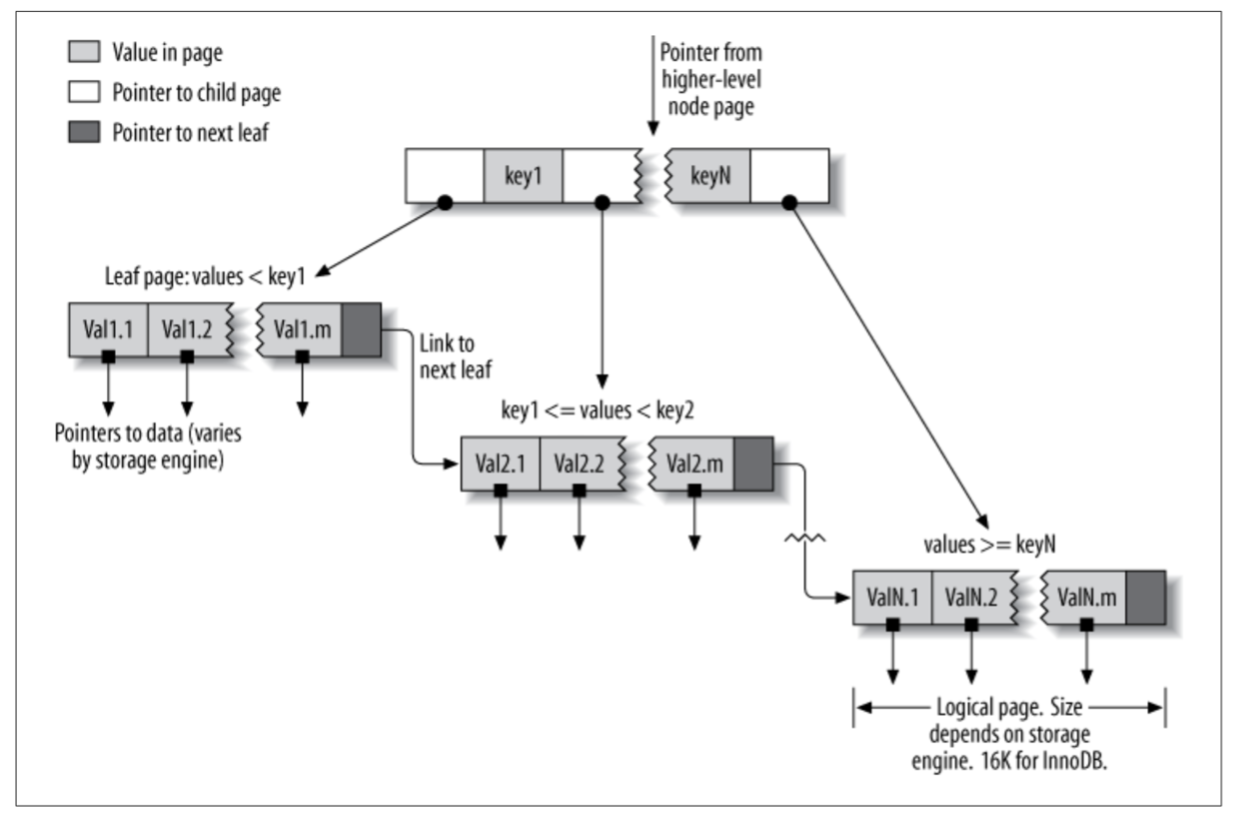
\includegraphics[width=.8\textwidth]{PNGs/Index/B_Tree_Visualisation}
    \caption[Binärbaum - Grafik]{Darstellung des binären Baums mit Knoten und Blättern}
    \label{fig:b-tree-visualisation}
\end{figure}

Blattseiten sind besonders, da sie Zeiger auf die indexierten Daten enthalten, anstatt auf andere Seiten zu verweisen.
Zwischen dem Wurzelknoten und den Blattseiten können viele Ebenen von Knoten-Seiten existieren.
Die Tiefe des Baumes hängt von der Größe der Tabelle ab.

Außerdem speichern B-Bäume die indexierten Spalten in einer festgelegten Reihenfolge, was sie besonders nützlich für die Suche nach Datenbereichen macht.
Beispielsweise kann ein Index auf einem Textfeld (z.B. vom Typ \texttt{VARCHAR}) effizient alle Namen finden, die mit „K“ beginnen, da die Werte in alphabetischer Reihenfolge gespeichert sind.

Der Index sortiert die Werte entsprechend der Reihenfolge der in der \texttt{CREATE TABLE}-Anweisung angegebenen Spalten, beispielsweise des Primärschlüssels (\texttt{last\_name, first\_name, b\_day}).
B-Baum-Indizes eignen sich gut für Suchen mit dem vollständigen Schlüsselwert (engl. full key value), einem Schlüsselbereich (engl. key range) oder einem Schlüsselpräfix (engl. full key prefix).
Beim Schlüsselpräfix ist dies jedoch nur der Fall, wenn die Suche das linkeste Präfix des Indexes verwendet.

Als nächstes betrachten wir die möglichen Abfragen, bei denen B-Baum-Indizes besonders hilfreich sind, um ein besseres Verständnis für ihre optimale Nutzung zu erlangen.
Eine Übereinstimmung mit dem vollständigen Schlüsselwert liefert Werte für alle Spalten im Index.
Eine beispielhafte Abfrage wäre die Suche nach allen Einträgen für Max Mustermann, geboren am 2000-01-01, wenn der Schlüssel aus Nachname, Vorname und Geburtsdatum besteht.
Für diesen Index sind auch Abfragen nützlich, die nur mit dem linken Präfix übereinstimmen, beispielsweise die Suche nach „Mustermann“.
Eine weitere Möglichkeit ist die Übereinstimmung mit einem Spaltenpräfix, also dem ersten Teil eines Spaltenwerts, etwa alle Nachnamen, die mit „M“ beginnen.
Ebenso effizient ist der Index bei der Übereinstimmung mit einem Wertebereich, z.B. Nachnamen zwischen „Mustermann“ und „Müller“.

Ein B-Baum-Index kann auch genutzt werden, um Abfragen effizient zu unterstützen, bei denen eine Spalte exakt und eine andere innerhalb eines Wertebereichs abgefragt wird.
Beispielsweise könnte dies eine exakte Übereinstimmung mit dem Nachnamen „Mustermann“ und eine Bereichsabfrage für Vornamen, die mit „Ma“ beginnen, umfassen.
Der letzte Anwendungsfall sind Abfragen, die nur den Index verwenden und nicht die gespeicherten Zeilen, etwa wenn alle benötigten Daten im Index enthalten sind.

Ein weiterer Vorteil von B-Baum-Indizes ist, dass sie aufgrund der sortierten Baumstruktur nicht nur Abfragen, sondern auch \texttt{ORDER BY}-Bedingungen effizient unterstützen können.
Wenn ein B-Baum für die Suche genutzt werden kann, kann er auch für die Sortierung der Ergebnisse verwendet werden.

Es gibt jedoch Einschränkungen von B-Baum-Indizes, die dazu führen, dass andere Indextypen für bestimmte Szenarien besser geeignet sind.
Eine Einschränkung ist, dass die Suche nicht am linken Ende des Indexes beginnen kann.
Beispielsweise ist ein Index, der aus Nachname, Vorname und Geburtsdatum besteht, nicht geeignet, um alle Personen zu finden, die vor dem Jahr 2000 geboren wurden, ohne dass der Nachname und Vorname ebenfalls spezifiziert werden.

Für optimale Leistung sollten Indizes mit den gleichen Spalten, jedoch in unterschiedlicher Reihenfolge erstellt werden, um die häufigsten Abfragen zu optimieren.
Eine Analyse der am häufigsten verwendeten Abfragen kann dabei helfen zu entscheiden, ob zusätzliche Indizes erforderlich sind.


\begin{figure}[!ht]
    \centering
    \begin{subfigure}[t]{0.48\textwidth}
        \centering
        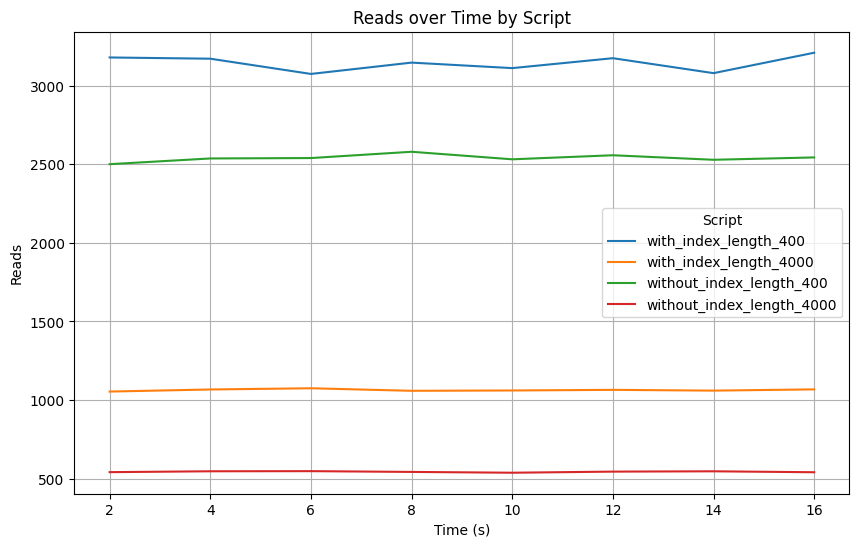
\includegraphics[width=\textwidth]{PNGs/Script/Index/B_Tree/high-count/Reads}
        \label{high-reads}
    \end{subfigure}
    \hfill
    \begin{subfigure}[t]{0.48\textwidth}
        \centering
        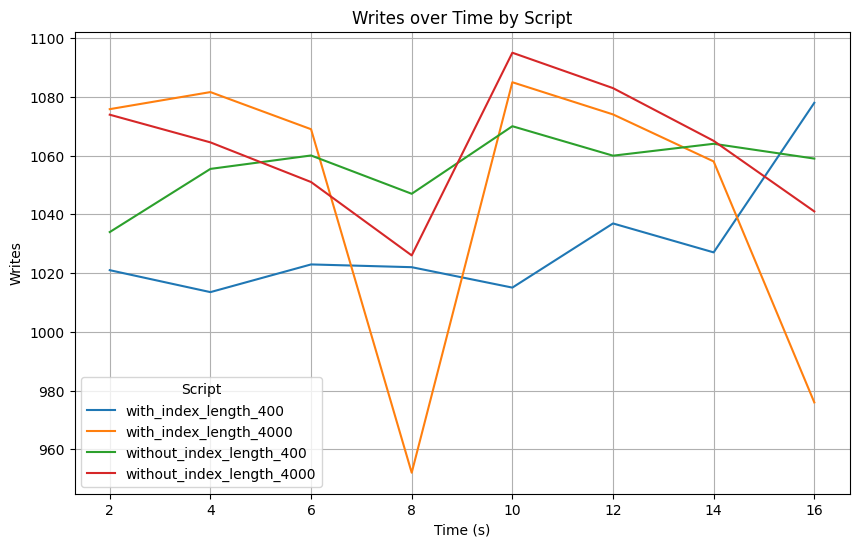
\includegraphics[width=\textwidth]{PNGs/Script/Index/B_Tree/high-count/Writes}
        \label{high-writes}
    \end{subfigure}
    \caption[High-Counts: Reads und Writes]{Grafik zeigt die verschiedenen Zeiten (in ms) für Readsabfragen (links) und Schreibbefehle (rechts) mit 500 bzw. 5000 Zeilen}
    \label{fig:high-b-tree-columns}
\end{figure}

\begin{figure}[!ht]
    \centering
    \begin{subfigure}[t]{0.48\textwidth}
        \centering
        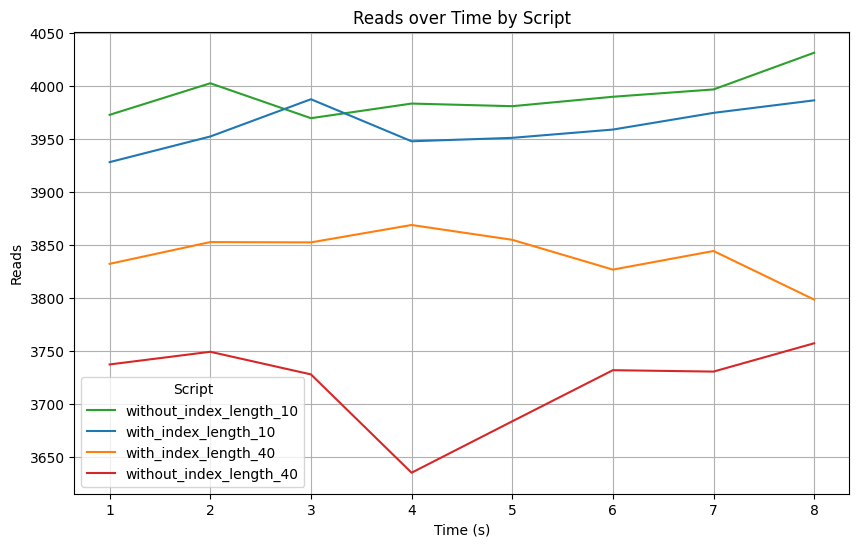
\includegraphics[width=\textwidth]{PNGs/Script/Index/B_Tree/low-count/Reads}
        \label{low-reads}
    \end{subfigure}
    \hfill
    \begin{subfigure}[t]{0.48\textwidth}
        \centering
        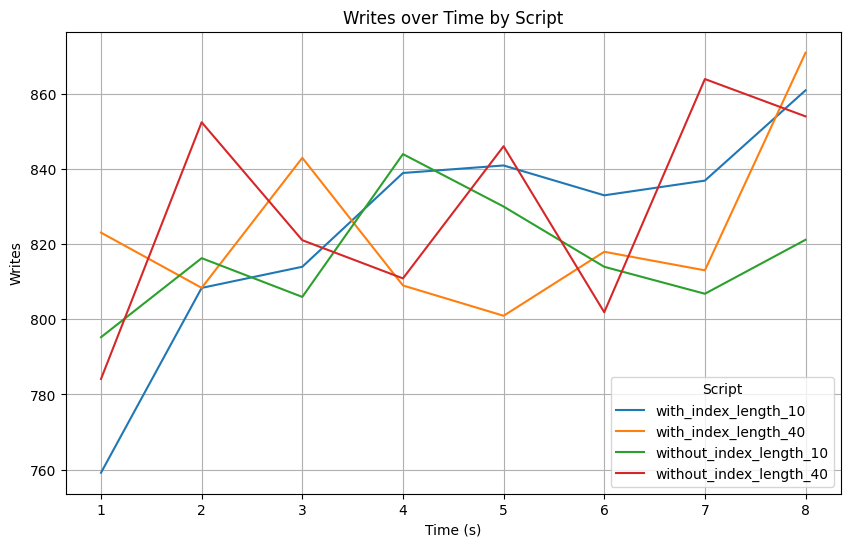
\includegraphics[width=\textwidth]{PNGs/Script/Index/B_Tree/low-count/Writes}
        \label{low-writes}
    \end{subfigure}
    \caption[Low-Counts: Reads und Writes]{Grafik zeigt die verschiedenen Zeiten (in ms) für Readsabfragen (links) und Schreibbefehle (rechts) mit 10 bzw. 100 Zeilen dar}
    \label{fig:low-b-tree-columns}
\end{figure}

\begin{figure}[!ht]
    \centering
    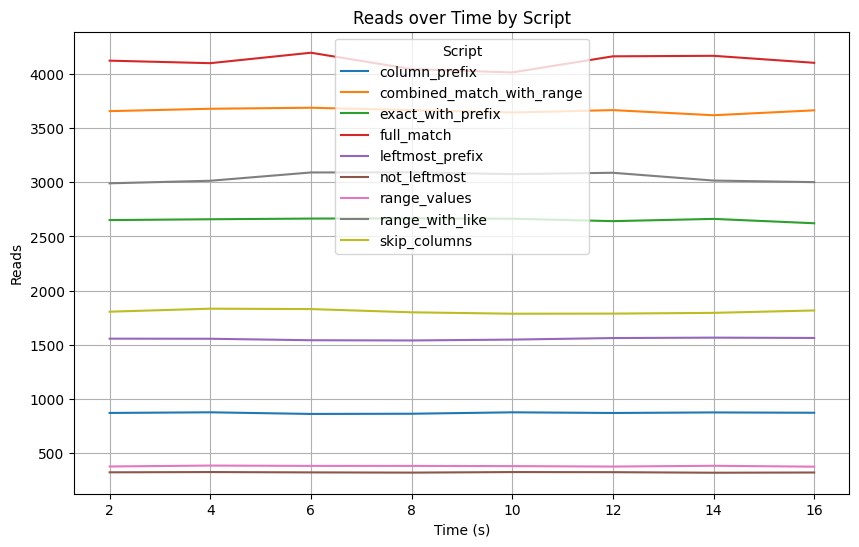
\includegraphics[width=.8\textwidth]{PNGs/Script/Index/B_Tree/b-tree-query-differences/Reads}
    \caption[B - Tree - Selects - Ergebnis]{Grafik visualisiert die Unterschiede von verschieden Select - Queries auf dieselben Daten. Je nach Gewschiwndikeit greift der Index besser oder nicht }
    \label{fig:b-tree-query-reads}
\end{figure}


\section{Hash - Index}
Ein weiterer Indextyp, den wir betrachten, ist der Hash-Index.
Dieser basiert auf einer Hash-Tabelle und ist daher nur für exakte Suchanfragen geeignet, die alle Spalten im Index verwenden.
Die Funktionsweise der Storage-Engine lässt sich wie folgt beschreiben: Für jede Zeile wird mithilfe einer Hash-Funktion ein Hash-Wert der indexierten Spalte berechnet.
Der Hash-Wert (engl.\textit{hash code}) ist eine kleine Zahl, die sich in der Regel von den Hash-Werten anderer Zeilen mit unterschiedlichen Schlüsselwerten unterscheidet.


In MySQL unterstützt nur die Memory-Storage-Engine explizite Hash-Indizes.
Der bereits besprochene Standard-Indextyp für Memory-Tabellen, der B-Baum-Index, ist jedoch ebenfalls möglich.
Außerdem unterstützt die Memory-Engine keine eindeutigen Hash-Indizes.
Das bedeutet, wenn mehrere Werte denselben Hash-Wert besitzen, speichert der Index die Zeiger auf die Zeilen (engl. \textit{row pointers}) in demselben Hash-Tabelleneintrag, typischerweise mithilfe einer verketteten Liste (z.B. einer \textit{Linked List}).
Im Gegensatz dazu stellen eindeutige Hash-Indizes sicher, dass für jeden Hash-Wert nur ein einziger Eintrag existiert.
Bei Konflikten wird ein Mechanismus wie die \textit{Open Addressing}-Strategie (z.B. \textit{Linear Probing} oder \textit{Quadratic Probing}) eingesetzt, um Konflikte zu lösen und den Speicherplatz effizient zu verwalten.
Hierbei wird versucht, Konflikte direkt innerhalb der Hash-Tabelle zu bewältigen, anstatt auf zusätzliche Datenstrukturen wie verkettete Listen zurückzugreifen.

Um die Berechnung der Hash-Funktion genauer zu erläutern, folgt ein Beispiel:

\begin{lstlisting}[language=SQL,caption=Variationen,label=select-query-hash]
SELECT lname FROM testhash WHERE fname = 'Peter';
\end{lstlisting}

Zunächst berechnet MySQL den Hash-Wert für \texttt{'Peter'} und verwendet diesen, um den entsprechenden Zeiger im Index zu finden.
Angenommen, die Hash-Funktion liefert für \texttt{'Peter'} den Wert \textbf{7654}.
MySQL sucht nun im Index an der Position 7654 und findet einen Zeiger auf Zeile 3.
Im letzten Schritt wird der Wert in Zeile 3 mit \texttt{'Peter'} verglichen, um sicherzustellen, dass es sich um die richtige Zeile handelt.
Da die Indizes nur kompakte Hash-Werte speichern, sind Hash-Indizes äußerst platzsparend, und Suchvorgänge erfolgen in hoher Geschwindigkeit.

Ähnlich wie der B-Baum-Index hat auch der Hash-Index einige Einschränkungen, auf die wir nun eingehen:

Da der Index nur Hash-Werte und Zeiger auf Zeilen (engl. \textit{row pointers}) enthält, jedoch nicht die Werte selbst, kann MySQL den Index nicht verwenden, um das Einlesen der Zeilen zu vermeiden.
Da der Zugriff auf die in den Speicher geladenen Zeilen jedoch sehr schnell ist, wird die Leistung dadurch nicht wesentlich beeinträchtigt.

Ein wesentlicher Nachteil von Hash-Indizes ist, dass sie nicht für Sortierungen verwendet werden können, da die Werte nicht in einer geordneten Reihenfolge gespeichert sind.
Im Gegensatz dazu können B-Baum-Indizes Sortierungen unterstützen, wenn sie entsprechend erstellt und genutzt werden.

Darüber hinaus ermöglichen Hash-Indizes keine partiellen Schlüsselübereinstimmungen (engl. \textit{partial key matching}).
Da der Hash-Wert aus dem gesamten indexierten Wert berechnet wird, hilft ein Hash-Index beispielsweise nicht, wenn ein Index aus den Spalten (A, B) besteht und die \texttt{WHERE}-Klausel nur auf A verweist.


Ein weiterer Nachteil besteht darin, dass Hash-Indizes keine Bereichsabfragen (engl. \textit{range queries}) unterstützen.
Sie eignen sich lediglich für Gleichheitsvergleiche, wie die Operatoren \texttt{=} (gleich), \texttt{<=>} (null-sicher gleich) und \texttt{IN()}.


Obwohl Hash-Indizes sehr performant sind, können Hash-Kollisionen ihre Leistung beeinträchtigen.
Wenn viele Werte denselben Hash-Wert aufweisen, muss die Storage-Engine jeden Zeiger in der verketteten Liste durchlaufen und die entsprechenden Werte mit dem Suchwert vergleichen, um die richtige(n) Zeile(n) zu finden.


Auch Index-Wartungsoperationen können bei vielen Kollisionen langsamer werden.
Wenn beispielsweise ein Index auf einer Spalte mit sehr geringer Selektivität erstellt wird und eine Zeile gelöscht werden soll, kann das Finden des entsprechenden Zeigers im Index sehr aufwendig sein, was auch das Löschen der Zeile verzögert.


Einige Speicher-Engines, wie beispielsweise InnoDB, können zudem erkennen, wenn bestimmte Index-Werte besonders häufig verwendet werden, und automatisch einen Hash-Index für diese Werte im Speicher (engl.\textit{memory}) erstellen, der zusätzlich zu den vorhandenen B-Baum-Indizes genutzt wird.


\begin{figure}[!ht]
    \centering
    \begin{subfigure}[t]{0.48\textwidth}
        \centering
        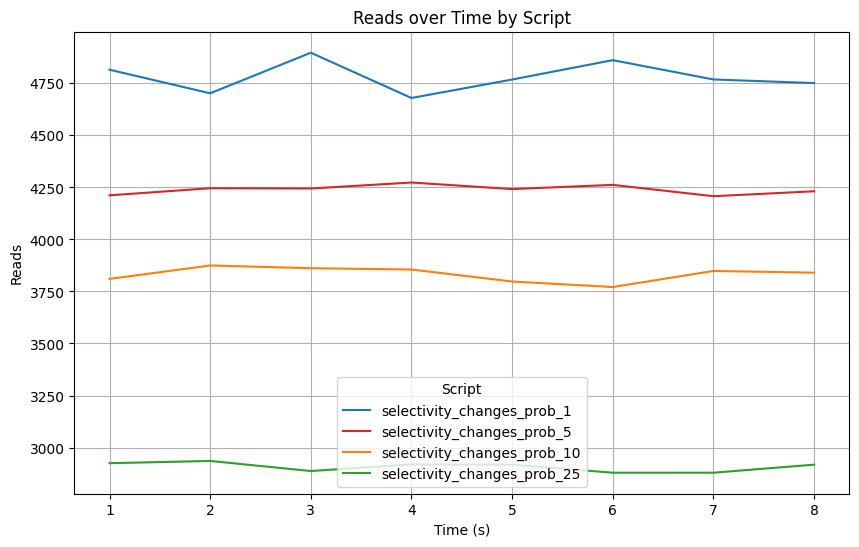
\includegraphics[width=\textwidth]{PNGs/Script/Index/Hash/selectivity-change/Reads}
        \caption[Hash - Kollisionen - Reads - Ergebnis]{Unterschiede von Readsabfragen}
        \label{hash-collision-reads}
    \end{subfigure}
    \hfill
    \begin{subfigure}[t]{0.48\textwidth}
        \centering
        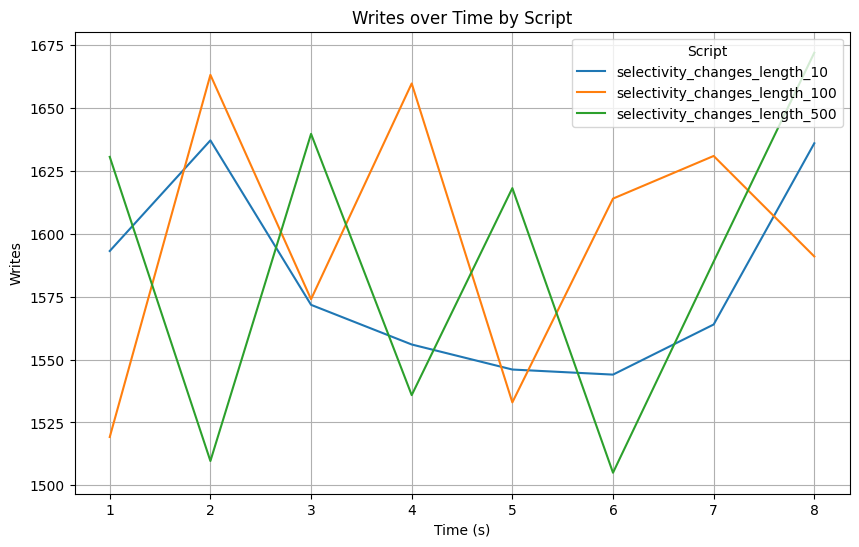
\includegraphics[width=\textwidth]{PNGs/Script/Index/Hash/selectivity-change/Writes}
        \caption[Hash - Kollisionen - Writes - Ergebnis]{Unterschiede von Schreibbefehlen}
        \label{hash-collision-writes}
    \end{subfigure}
    \caption[Hash-Kollisionen: Reads und Writes]{Vergleich der Auswirkungen von Hashkollisionen auf Lese- und Schreibvorgänge in Abhängigkeit von der Anzahl an Hashkollisionen.}
    \label{fig:hash-collision-comparison}
\end{figure}

\begin{figure}[!ht]
    \centering
    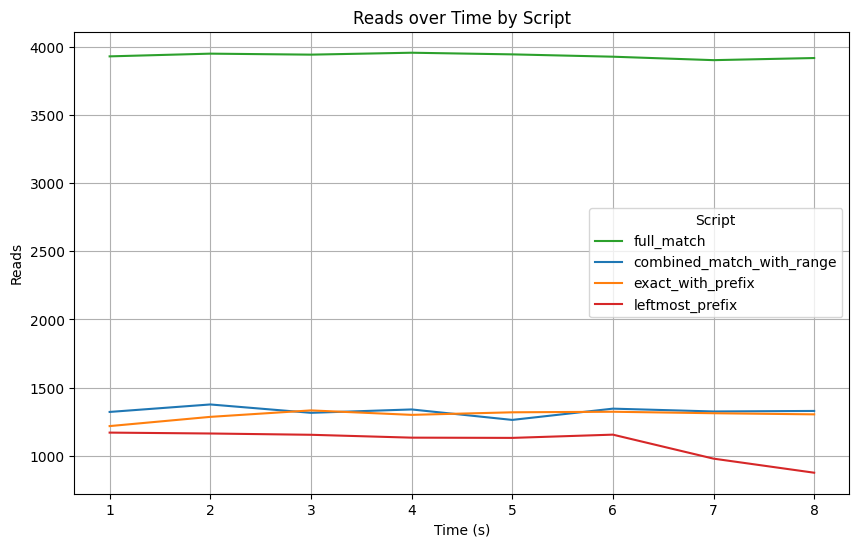
\includegraphics[width=.8\textwidth]{PNGs/Script/Index/Hash/hash-query-differences/Reads}
    \caption[Hash - Selects - Ergebnis]{Grafik visualisiert die Unterschiede von verschieden Select - Queries auf dieselben Daten. Je nach Gewschiwndikeit greift der Index besser oder nicht }
    \label{fig:hash-query-reads}
\end{figure}